\documentclass[aspectratio=169]{beamer}

\mode<presentation>
\usetheme{Boadilla}
\definecolor{Khaki}{RGB}{144,110,62}
\definecolor{blue}{RGB}{30,90,205}
\definecolor{red}{RGB}{213,94,0}
\definecolor{green}{RGB}{0,128,0}
\setbeamercolor{title}{fg=Khaki}
\setbeamercolor{frametitle}{fg=Khaki}
\setbeamercolor{block title}{bg=Khaki, fg=white}
\setbeamercolor{block body}{bg=white}
\setbeamercolor{structure}{fg=Khaki}
\setbeamercolor{item projected}{fg=white}
\setbeamercolor{item}{fg=Khaki}
\setbeamercolor{subitem}{fg=Khaki}
\setbeamercolor{section in toc}{fg=Khaki}
\setbeamercolor{description item}{fg=Khaki}
\setbeamercolor{caption name}{fg=Khaki}
\setbeamercolor{button}{bg=Khaki, fg=white}
\setbeamercolor{caption name}{fg=Khaki}
\usepackage{graphics}
\usepackage{tikz}
\usepackage{amsmath}
\usepackage{bbm}
\usetikzlibrary{decorations.pathreplacing}
\usepackage{geometry}
\usepackage{booktabs}
\usepackage{bookmark}
\usepackage{multirow, makecell}
\usepackage{float}
\usepackage{fancyvrb}
\usepackage{caption}
\usepackage{subcaption}
\usepackage{adjustbox}
\usepackage{hyperref}
\usepackage{threeparttable}
\usepackage{appendixnumberbeamer} 
\usepackage[T1]{fontenc}
\usepackage[default]{lato} 

\newenvironment{wideitemize}{\itemize\addtolength{\itemsep}{10pt}}{\enditemize}
\newenvironment{wideenumerate}{\enumerate\addtolength{\itemsep}{10pt}}{\endenumerate}
\newenvironment{widedescription}{\description\addtolength{\itemsep}{10pt}}{\enddescription}
\hypersetup{
colorlinks=true,
linkcolor=black,
filecolor=green, 
urlcolor=blue,
}
\beamertemplatenavigationsymbolsempty
\setbeamercolor{author in head/foot}{bg=white, fg=Khaki}
\setbeamercolor{title in head/foot}{bg=white, fg=Khaki}
\setbeamercolor{date in head/foot}{bg=white, fg=Khaki}
\setbeamercolor{section in head/foot}{bg=white, fg=Khaki}
\setbeamercolor{page number in head/foot}{bg=white, fg=Khaki}
\setbeamercolor{headline}{bg=white}
\setbeamertemplate{footline}{
    \leavevmode%
    \hbox{%
        \begin{beamercolorbox}[wd=.33\paperwidth,ht=2.25ex,dp=1ex,center]{date in head/foot}%
            \usebeamerfont{date in head/foot}\insertshortdate
        \end{beamercolorbox}%
        \begin{beamercolorbox}[wd=.44\paperwidth,ht=2.25ex,dp=1ex,center]{title in head/foot}%
            \usebeamerfont{title in head/foot}\insertshorttitle
        \end{beamercolorbox}%
        \begin{beamercolorbox}[wd=.22\paperwidth,ht=2.25ex,dp=1ex,center]{page number in head/foot}%
            \usebeamerfont{page number in head/foot}\insertframenumber{} / \inserttotalframenumber
        \end{beamercolorbox}}%
        \vskip0pt%
    }
%\setbeamercolor{page number in head/foot}{fg=black}
\setbeamertemplate{section in toc}[sections numbered]
\setbeamertemplate{subsection in toc}{\leavevmode\leftskip=3em\rlap{\hskip-1.75em\inserttocsectionnumber.\inserttocsubsectionnumber}\inserttocsubsection\par}
\setbeamerfont{subsection in toc}{size=\footnotesize}

\newenvironment{transitionframe}{\setbeamercolor{background canvas}{bg=Khaki}\setbeamertemplate{footline}{} \begin{frame}}{\end{frame}}


\makeatletter
\let\@@magyar@captionfix\relax
\makeatother


\title[Recitation 3 (UN 3412)]{Recitation 3: OLS properties: Sampling distribution and fitness} % Change this regularly
\author[Lee]{Seung-hun Lee}
\institute[]{Columbia University \\ Undergraduate Introduction to Econometrics Recitation}

\date[September 29th, 2022]{September 29th, 2022}

\begin{document}
\begin{frame}
\titlepage
\end{frame}


%%% Color slides for section headers: Use for colloquium version (The ones bewteen \iffals and \fi)



\begin{transitionframe}
  \begin{center}
         { \Huge \textcolor{white}{Ordinary least squares}}
       \end{center}
\end{transitionframe}

\begin{frame}
\frametitle{Ordinary Least Squares: Population vs sample linear models}
\begin{itemize}
\item Suppose that the \textbf{population linear regression model} (also known as data generating process in some books) is
\[
Y_i = \beta_0 + \beta_1X_i + u_i
\]
\item However, we do not know the true values of the population parameters - $\beta_0$ and $\beta_1$
\item An alternative way to approach the problem is to use the \textbf{sample linear regression model} (or just model)
\[
Y_i = \hat{\beta}_0 +\hat{\beta}_1X_i +\hat{u}_i
\]
where $\hat{\beta}_0, \hat{\beta}_1$ are estimates of ${\beta}_0, {\beta}_1$

\end{itemize}
\end{frame}

\begin{frame}
\frametitle{Ordinary Least Squares: Definition}
\begin{itemize}
\item The ideal estimator minimizes the squared sum of residuals. 
\item Mathematically, this can be obtained by solving the following minimization problem and the first order conditions
\footnotesize{\begin{gather*}
\min_{\hat{\beta}_0, \hat{\beta}_1} \sum_{i=1}^n (Y_i-\hat{\beta}_0 - \hat{\beta}_1X_i)^2\\
[\hat{\beta}_0]: -2\sum_{i=1}^n(Y_i-\hat{\beta}_0-\hat{\beta}_1X_i)=0\\
[\hat{\beta}_1]: -2\sum_{i=1}^nX_i(Y_i-\hat{\beta}_0-\hat{\beta}_1X_i)=0 
\end{gather*}}\normalsize
The resulting \textbf{least squares estimators} are
\[
\hat{\beta}_0 = \bar{Y}-\hat{\beta}_1\bar{X}, \ \ \hat{\beta}_1=\frac{\sum_{i=1}^n(Y_i-\bar{Y})(X_i-\bar{X})}{\sum_{i=1}^n(X_i-\bar{X})^2}
\]
\end{itemize}
\end{frame}


\begin{frame}
\frametitle{Ordinary Least Squares: Main assumptions}
\begin{itemize}
\item For OLS to be unbiased, consistent, efficient, and asymptotic normal, the following assumptions must be made
\begin{block}{Assumptions}
\begin{itemize}
\item[\textbf{A0}] Linearity: The regression is assumed to be linear in parameters.
\[
\text{Okay: } Y_i = \beta_0 + \beta_1X_i + \beta_2X_i^2+u_i, \ \text{Not: } Y_i = \beta_0 + \beta_1X_i + \beta_2^2X_i+u_i
\]
\item[\textbf{A1}] $E(u_i|X_i)=0$: Conditional on letting $X_i$ take a certain value, we are not making any systematical error in the linear regression. This is required for the OLS to be unbiased. (or $cov(X_i, u_i)=0$)
\item[\textbf{A2}] i.i.d. (random sampling): $(X_i,Y_i)$ is assumed to be from independent, identical distribution
\item[\textbf{A3}] No Outliers: Outlier has no impact on the regression results. ($E(X_i^4), E(Y_i^4)<\infty$)
\item[\textbf{A4}] Homoskedasticity: $var(u_i)=\sigma_u$ (variance of $u_i$ does not depend on $X_i$). $\leftrightarrow$ \textit{heteroskedasticity}
\item[\textbf{A5}] No Autocorrelation (Serial Correlation): For $i\neq j$, $cov(u_i,u_j)=0$. Error at the previous period does not have any impact on the current period. This is usually broken in time series settings

\end{itemize}
\end{block}
\end{itemize}
\end{frame}


\begin{frame}
\frametitle{Ordinary Least Squares: Useful alternative expression for $\hat{\beta}_1$ }
\begin{itemize}
\item OLS estimate that we are getting is a random variable - getting different estimates depending on sample we work with. 
\item$\hat{\beta}_1$: Recall that we can write
\[
\hat{\beta}_1= \frac{\sum_{i=1}^n(X_i-\bar{X})(Y_i-\bar{Y})}{\sum_{i=1}^n(X_i-\bar{X})^2}
\]
Now, replace $Y_i$ an $\bar{Y}$ with 
\[
Y_i =\beta_0 + \beta X_i + u_i, \ \bar{Y} = \beta_0 + \beta_1\bar{X} + \bar{u},
\]
which allows us to write 
\[
(Y_i-\bar{Y}) = (\beta_1(X_i-\bar{X})+(u_i-\bar{u}))
\]
and get
\[
\hat{\beta}_1=\beta_1+  \frac{\sum_{i=1}^n(X_i-\bar{X})(u_i-\bar{u})}{\sum_{i=1}^n(X_i-\bar{X})^2}
\]

\end{itemize}
\end{frame}


\begin{frame}
\frametitle{Ordinary Least Squares: Unbiasedness of $\hat{\beta}_1$}
\begin{itemize}
\item $E[\hat{\beta}_1]$: It can be written as
\small{\[
\begin{aligned}
E[\hat{\beta}_1]& = E\left[\beta_1+  \frac{\sum_{i=1}^n(X_i-\bar{X})(u_i-\bar{u})}{\sum_{i=1}^n(X_i-\bar{X})^2}\right]\\
&=\beta_1+ E\left[\frac{\sum_{i=1}^n(X_i-\bar{X})(u_i-\bar{u})}{\sum_{i=1}^n(X_i-\bar{X})^2}\right]
\end{aligned}
\]}\normalsize
$\sum_{i=1}^n(X_i-\bar{X})(u_i-\bar{u})$ can be written to something simpler.
\small{\[
\sum_{i=1}^n(X_i-\bar{X})(u_i-\bar{u})=\sum_{i=1}^nX_iu_i-\bar{u}\sum_{i=1}^n X_i-\bar{X}\sum_{i=1}^nu_i+n\bar{X}\bar{u} = \sum_{i=1}^n(X_i-\bar{X})u_i
\]}\normalsize
\item[$\to$] Since $\bar{X}$ is a sample mean of $X$, $\sum_{i=1}^nX_i=n\bar{X}$. \\
\item[$\to$] The assumption that conditional mean is zero and $(X_i, u_i)$ are uncorrelated means that the term on the left hand side is zero. 
\item[$\to$] Therefore, UNDER CLASSICAL ASSUMPTIONS, $E[\hat{\beta}_1]=\beta_1$.

\end{itemize}
\end{frame}


\begin{frame}
\frametitle{Ordinary Least Squares: Unbiasedness of $\hat{\beta}_0$}
\begin{itemize}
\item $\hat{\beta}_0$: The formula for $\hat{\beta}_0$ is $\bar{Y}-\hat{\beta}_1\bar{X}$. By changing $\bar{Y}$, we can get
\[
\begin{aligned}
\hat{\beta}_0&=(\beta_0+\beta_1\bar{X}+\bar{u})-\hat{\beta}_1\bar{X}\\
&=\beta_0+(\beta_1-\hat{\beta}_1)\bar{X}+\bar{u}
\end{aligned}
\]
Then we can say the following about the sampling distribution
\item $E[\hat{\beta}_0]$: We can write
\[
E[\hat{\beta}_0]=\beta_0+E[(\beta_1-\hat{\beta}_1)\bar{X}]+E[\bar{u}]=\beta_0
\]
since $\hat{\beta}_1$ is unbiased and conditional expectation of $u_i$ is zero. 
\item[$\to$]Thus, under our current assumptions, $\hat{\beta}_0$ is unbiased. 
\end{itemize}
\end{frame}

\begin{frame}
\frametitle{Ordinary Least Squares: Variances of $\hat{\beta}_0$ and $\hat{\beta}_1$}
\begin{itemize}
\item Might take bit of a work, but when you follow the notes, you get
\[
var(\hat{\beta}_0)= \frac{\sigma_u^2}{n}\frac{\sum_{i=1}^nX_i^2}{\sum_{i=1}^n(X_i-\bar{X})^2}, var(\hat{\beta}_1)=\frac{\sigma_u^2}{\sum_{i=1}^n(X_i-\bar{X})^2}
\]
\item At the end of the day, we can say
\begin{gather*}
 \hat{\beta}_1 \sim N\left(\beta_1, \frac{\sigma_u^2}{\sum_{i=1}^n(X_i-\bar{X})^2}\right) \\
\hat{\beta}_0 \sim N\left(\beta_0, \frac{\sigma_u^2}{n}\frac{\sum_{i=1}^nX_i^2}{\sum_{i=1}^n(X_i-\bar{X})^2}\right)
\end{gather*}
\item The importance of this is that now we can conduct a hypothesis test and create a test statistic based on this distribution
\end{itemize}
\end{frame}

\begin{frame}
\frametitle{Ordinary Least Squares: How well does the model capture the data?}
Measure of fitness
\begin{itemize}
\item These numbers tell us how informative the sample linear regression we used is in telling us about the population data
\item $\mathbf{R^2}$: It is defined as a fraction of total variation which is explained by the model. Mathematically, this is
\footnotesize{%
\begin{gather*} 
Y_i = \underbrace{\hat{\beta}_0 + \hat{\beta}_1X_i}_{\hat{Y}_i} + u_i, \ \bar{Y} = \underbrace{\hat{\beta}_0 + \hat{\beta}_1\bar{X}}_{\bar{\hat{Y}}} + \bar{u}, \\
\implies Y_i-\bar{Y} = (\hat{Y}_i - \bar{\hat{Y}}) - (u_i - \bar{u}) \\
\implies \sum_{i=1}^n (Y_i-\bar{Y})^2= \sum_{i=1}^n (\hat{Y}_i - \bar{\hat{Y}})^2+\sum_{i=1}^n(u_i - \bar{u})^2 - 2\sum_{i=1}^n(\hat{Y}_i - \bar{\hat{Y}}) (u_i - \bar{u})
\end{gather*}}\normalsize
\end{itemize}
\end{frame}

\begin{frame}
\frametitle{Ordinary Least Squares: Getting to $R^2$}
\begin{itemize}
\item Note that 
\footnotesize{\[
\sum_{i=1}^n(\hat{Y}_i - \bar{\hat{Y}}) (u_i - \bar{u})=\sum_{i=1}^n\hat{Y}_i{u}_i-\bar{\hat{Y}}\sum_{i=1}^nu_i -\bar{u}\sum_{i=1}^n\hat{Y}_i +n\bar{u}\bar{\hat{Y}}
\]}\normalsize
\item Since $\sum_{i=1}^nu_i = n\bar{u},\ \sum_{i=1}^n\hat{Y}_i = n\bar{\hat{Y}}$ and $\sum_{i=1}^n\hat{Y}_iu_i=n\bar{u}\bar{\hat{Y}}$, all terms cancel each other out. 
\item So we are left with
\footnotesize{\begin{gather*}
\underbrace{\sum_{i=1}^n (Y_i-\bar{Y})^2}_{TSS}= \underbrace{\sum_{i=1}^n (\hat{Y}_i - \bar{\hat{Y}})^2}_{ESS}+\underbrace{\sum_{i=1}^n(u_i - \bar{u})^2}_{RSS} \\
\implies 1=\frac{\sum_{i=1}^n (\hat{Y}_i - \bar{\hat{Y}})^2}{\sum_{i=1}^n (Y_i-\bar{Y})^2} + \frac{\sum_{i=1}^n(u_i - \bar{u})^2 }{\sum_{i=1}^n (Y_i-\bar{Y})^2}
\end{gather*}}\normalsize
\end{itemize}
\end{frame}


\begin{frame}
\frametitle{Ordinary Least Squares: Getting to $R^2$}
\begin{itemize}
\item Thus, the $R^2$ can be found as
\[
R^2 = \frac{\sum_{i=1}^n (\hat{Y}_i - \bar{\hat{Y}})^2}{\sum_{i=1}^n (Y_i-\bar{Y})^2} = \frac{ESS}{TSS} = 1-\frac{RSS}{TSS}
\]
\item Intuitively, higher $R^2$ implies that the model explains more of the total variance, which implies that the regression fits the data well. 
\end{itemize}
\end{frame}


\begin{frame}
\frametitle{Ordinary Least Squares: Setting up  the hypothesis test}

\begin{itemize}
\item From the sample distribution of $\hat{\beta}_1$, we can break down into two cases
\item \textbf{Know $\sigma_u$}: Since the $\hat{\beta}_1$ takes a normal distribution, we can ``standardize" it to get the test statistic and the distribution for it
\[
\frac{\hat{\beta}_1-\beta_1}{\sqrt{var(\hat{\beta}_1)}}\sim N(0,1)
\]
and compare against the critical values (depending on significance level, two vs one-sided test)
\end{itemize}
\end{frame}

\begin{frame}
\frametitle{Ordinary Least Squares: Hypothesis test methods}

\begin{itemize}
\item \textbf{Don't know $\sigma_u$}; need to have an estimate for $var(\hat{\beta}_1)$ due to not knowing $\sigma_u$. The test statistics and its distribution is
\[
\frac{\hat{\beta}_1-\beta_1}{\sqrt{\widehat{var(\hat{\beta}_1)}}}\sim t_{n-2}
\]
where $\widehat{var(\hat{\beta}_1)}$ is the estimate for the variance and $t_{n-2}$ is a t-distribution with $n-2$ degrees of freedom.
\item The d.f. is determined by the number of observations, where 2 is subtracted because we are estimating $\beta_0$ and $\beta_1$ in the process.
\item When $n$ is large, t-distribution becomes similar to the normal distribution
\end{itemize}
\end{frame}

\begin{frame}
\frametitle{Ordinary Least Squares: Confidence interval}

\begin{itemize}
\item  \textbf{Confidence interval}: A 95\% confidence interval is a range of numbers that form a random interval that has a 95\% chance of including a (nonrandom) true value of a parameter. 
\item This can be obtained by inverting the rejection region that we have used in the critical value approach.
\footnotesize{\begin{gather*}
\Pr\left(-1.96\leq \frac{\hat{\beta}_1-\beta_1}{\sqrt{var(\hat{\beta}_1)}} \leq1.96\right)=0.95\\
\implies \Pr\left(\hat{\beta}_1-1.96\times\sqrt{var(\hat{\beta}_1)} \leq \beta_1 \leq\hat{\beta}_1+1.96\times\sqrt{var(\hat{\beta}_1)}\right)=0.95
\end{gather*}}\normalsize
\item  If they encompass the null test value, then we cannot reject the null hypothesis. Otherwise, we can reject the null. 
\end{itemize}
\end{frame}


\begin{frame}
\frametitle{Errors may have different distribution across observations}
\begin{itemize}
\item The assumption that $var(u_i)$ is constant may not hold. Thus, be open for heteroskedasticity
\item If we stick to homoskedasticity in this case, the standard errors are incorrectly estimated (usually underestimated)
\begin{figure}[H]
\centering
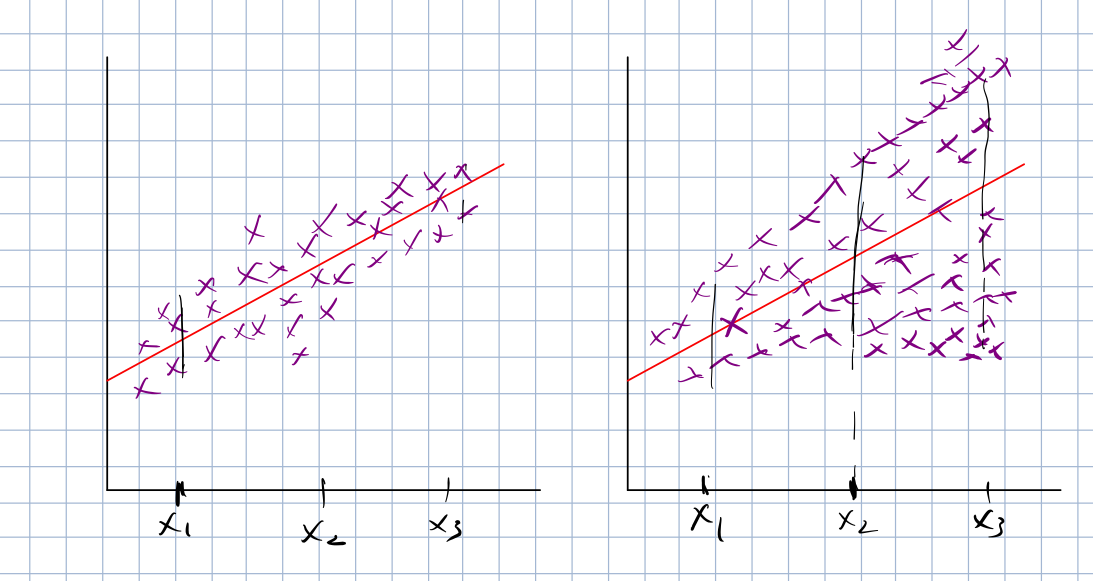
\includegraphics[width=0.55\textwidth]{hetero.png}
\end{figure}
\item  In such case, standard errors of our estimators must take this into account.
\end{itemize}
\end{frame}

\begin{frame}
\frametitle{...but what does heteroskedasticity change?}
\begin{figure}[H]
\centering
\begin{subfigure}[b]{0.49\textwidth}
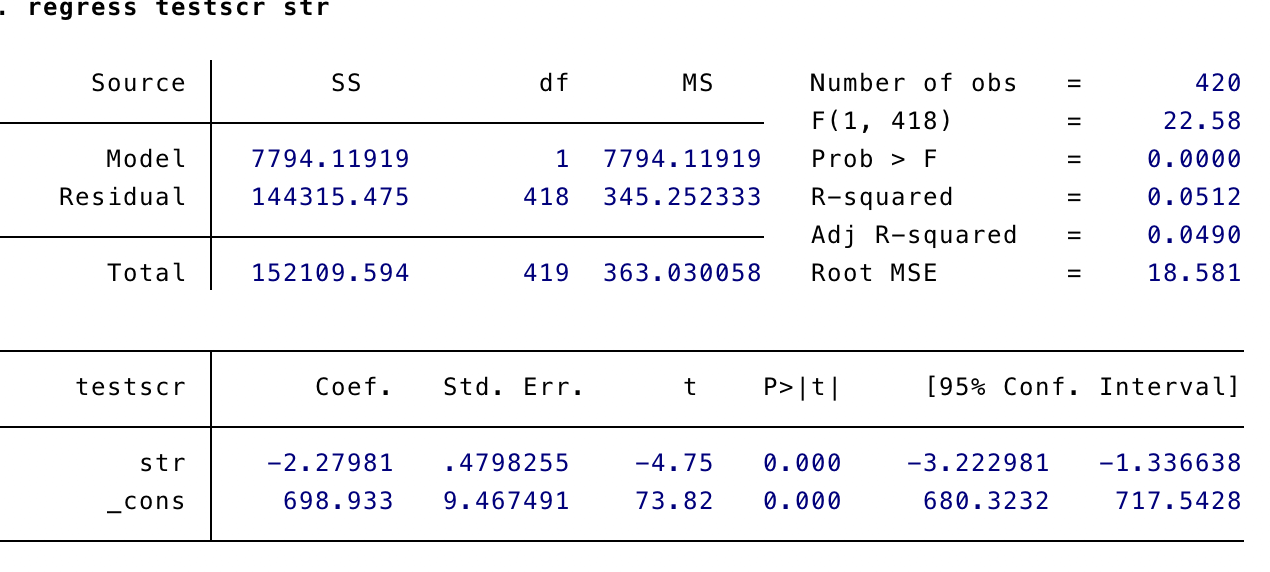
\includegraphics[width=\textwidth]{nonrobust.png}
\end{subfigure}
\begin{subfigure}[b]{0.49\textwidth}
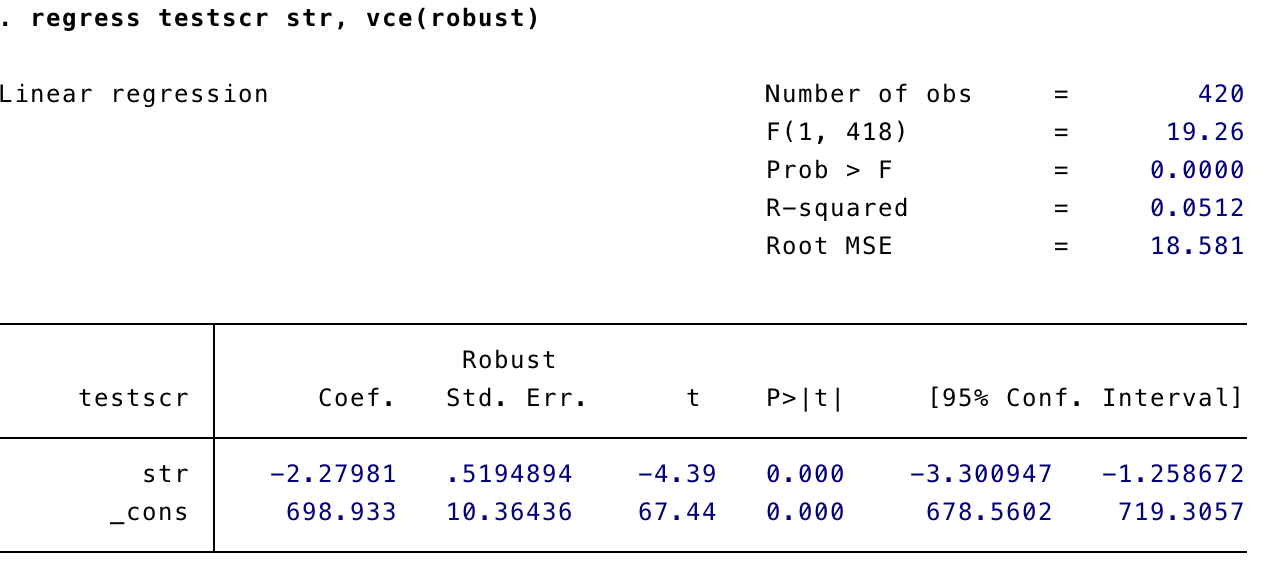
\includegraphics[width=\textwidth]{robust.png}
\end{subfigure}
\end{figure}
\begin{itemize}
\item The variance rises (usually) in the heteroskedastic regression, so we may make a wrong hypothesis test
\item The coefficients are unchanged, since estimation of OLS estimates did not rely on homoskedasticity
\end{itemize}
\end{frame}



%%%%%%%%%%%
\end{document}
